%
% taylor.tex -- Repetition Taylot-Reihen
%
% (c) 2021 Prof Dr Andreas Müller, OST Ostschweizer Fachhochschule
% Erstellt durch Roy Seitz
%
% !TeX spellcheck = de_CH
\bgroup

\begin{frame}[t]
  \setlength{\abovedisplayskip}{5pt}
  \setlength{\belowdisplayskip}{5pt}
  \frametitle{Beispiel $\sin(x)$}
  \ifthenelse{\boolean{presentation}}{\vspace{-20pt}}{\vspace{-8pt}}
  \begin{block}{Taylor-Approximationen von $\sin(x)$}
    \begin{align*}
      p_{
      \only<1>{0}
      \only<2>{1}
      \only<3>{2}
      \only<4>{3}
      \only<5>{4}
      \only<6>{5}
      \only<7->{n}
      }(x)
      &= 
      \uncover<1->{0}
      \uncover<2->{+ x}
      \uncover<3->{+ 0 \frac{x^2}{2!}}
      \uncover<4->{- 1 \frac{x^3}{3!}}
      \uncover<5->{+ 0 \frac{x^4}{4!}}
      \uncover<6->{+ 1 \frac{x^5}{5!}}
      \uncover<7->{+ \ldots}
      \uncover<8->{
        = \sum_{k=0}^{n/2} (-1)^{2k + 1}\frac{x^{2k+1}}{(2k+1)!}
      }
    \end{align*}
  \end{block}
  \begin{center}
    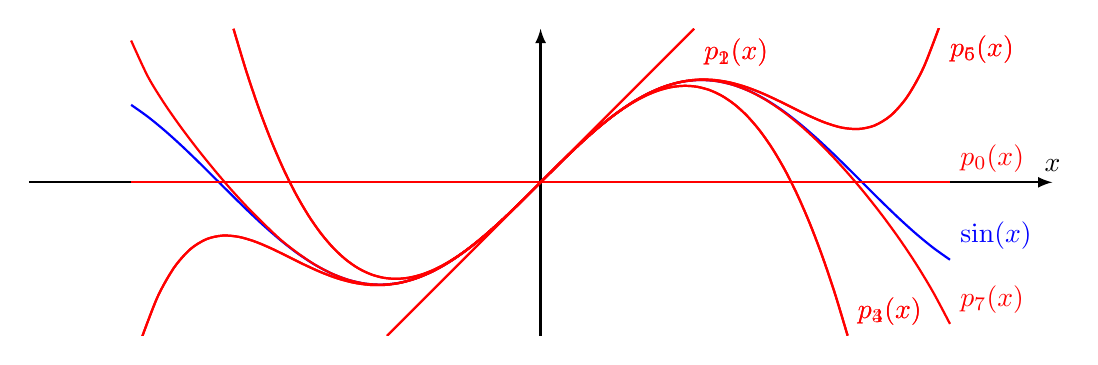
\begin{tikzpicture}[>=latex,thick,scale=1.3]
      \draw[->] (-5.0, 0.0) -- (5.0,0.0) coordinate[label=$x$];
      \draw[->] ( 0.0,-1.5) -- (0.0,1.5);
      \clip (-5,-1.5) rectangle (5,1.5);
      \draw[domain=-4:4, samples=50, smooth, blue]
      plot ({\x}, {sin(180/3.1415968*\x)})
      node[above right] {$\sin(x)$};
      \uncover<1|handout:0>{
        \draw[domain=-4:4, samples=2, smooth, red]
        plot ({\x}, {0})
        node[above right] {$p_0(x)$};}
      \uncover<2|handout:0>{
        \draw[domain=-1.5:1.5, samples=2, smooth, red]
        plot ({\x}, {\x})
        node[below right] {$p_1(x)$};}
      \uncover<3|handout:0>{
        \draw[domain=-1.5:1.5, samples=2, smooth, red]
        plot ({\x}, {\x})
        node[below right] {$p_2(x)$};}
      \uncover<4>{
        \draw[domain=-3:3, samples=50, smooth, red]
        plot ({\x}, {\x - \x*\x*\x/6})
        node[above right] {$p_3(x)$};}
      \uncover<5|handout:0>{
        \draw[domain=-3:3, samples=50, smooth, red]
        plot ({\x}, {\x - \x*\x*\x/6})
        node[above right] {$p_4(x)$};}
      \uncover<6|handout:0>{
        \draw[domain=-3.9:3.9, samples=50, smooth, red]
        plot ({\x}, {\x - \x*\x*\x/6 + \x*\x*\x*\x*\x/120})
        node[below right] {$p_5(x)$};}
      \uncover<7|handout:0>{
        \draw[domain=-3.9:3.9, samples=50, smooth, red]
        plot ({\x}, {\x - \x*\x*\x/6 + \x*\x*\x*\x*\x/120})
        node[below right] {$p_6(x)$};}
      \uncover<8-|handout:0>{
        \draw[domain=-4:4, samples=50, smooth, red]
        plot ({\x}, {\x - \x*\x*\x/6 + \x*\x*\x*\x*\x/120 -
          \x*\x*\x*\x*\x*\x*\x/5040})
        node[above right] {$p_7(x)$};}
    \end{tikzpicture}
  \end{center}
\end{frame}

\begin{frame}[t]
  \setlength{\abovedisplayskip}{5pt}
  \setlength{\belowdisplayskip}{5pt}
  \frametitle{Taylor-Reihen}
  \ifthenelse{\boolean{presentation}}{\vspace{-20pt}}{\vspace{-8pt}}
    \begin{block}{Polynom-Approximationen von $f(t)$}
      \begin{align*}
        p_n(t) 
        &=
        f(0)
        \uncover<2->{ + f' (0) t }
        \uncover<3->{ + f''(0)\frac{t^2}{2} }
        \uncover<4->{ + \ldots + f^{(n)}(0) \frac{t^n}{n!} }
        \uncover<5->{ = \sum_{k=0}^{n} f^{(k)} \frac{t^k}{k!} }
      \end{align*}
    \end{block}
  \uncover<6->{
    \begin{block}{Erste $n$ Ableitungen von $f(0)$ und $p_n(0)$ sind gleich!}}
    \begin{align*}
      \uncover<6->{ p'_n(t) }
      &
      \uncover<7->{
        = f'(0) 
        + f''(0)t 
        + \mathcal O(t^2)
      }
      &\uncover<8->{\Rightarrow}&&
      \uncover<8->{p'_n(0) = f'(0)}
      \\
      \uncover<9->{ p''_n(t) }
      &
      \uncover<10->{
        = f''(0) 
        + \mathcal O(t)
      }
      &\uncover<11->{\Rightarrow}&&
      \uncover<11->{ p''_n(0) = f''(0) }
    \end{align*}
  \end{block}
  \uncover<12->{
    \begin{block}{Für alle praktisch relevanten Funktionen $f(t)$ gilt:}
      \begin{align*}
        \lim_{n\to \infty} p_n(t)
        =
        f(t)
      \end{align*}
    \end{block}
  }
\end{frame}


\begin{frame}[t]
  \setlength{\abovedisplayskip}{5pt}
  \setlength{\belowdisplayskip}{5pt}
  \frametitle{Beispiel $e^t$}
  \ifthenelse{\boolean{presentation}}{\vspace{-20pt}}{\vspace{-8pt}}
  \begin{block}{Taylor-Approximationen von $e^{at}$}
    \begin{align*}
      p_{
        \only<1>{0}
        \only<2>{1}
        \only<3>{2}
        \only<4>{3}
        \only<5>{4}
        \only<6>{5}
        \only<7->{n}
      }(t)
      &=
      1
      \uncover<2->{+ a t}
      \uncover<3->{+ a^2 \frac{t^2}{2}}
      \uncover<4->{+ a^3 \frac{t^3}{3!}}
      \uncover<5->{+ a^4 \frac{t^4}{4!}}
      \uncover<6->{+ a^5 \frac{t^5}{5!}}
      \uncover<7->{+ a^6 \frac{t^6}{6!}}
      \uncover<8->{+ \ldots
                   = \sum_{k=0}^{n} a^k \frac{t^k}{k!}}
      \\
      &
      \uncover<9->{= \exp(at)}
    \end{align*}
  \end{block}
  \begin{center}
    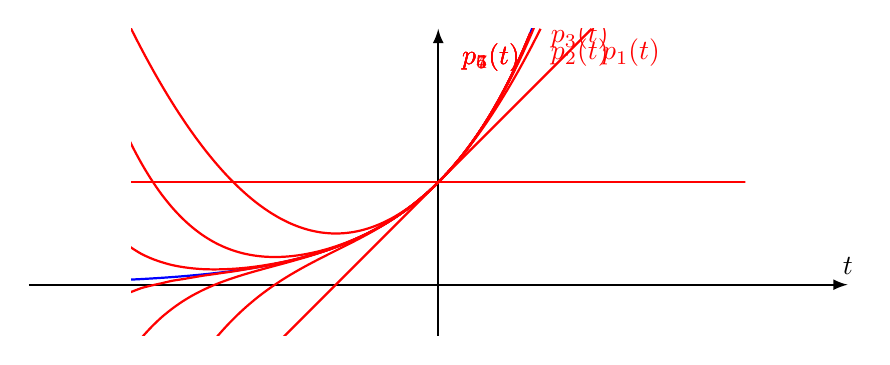
\begin{tikzpicture}[>=latex,thick,scale=1.3]
      \draw[->] (-4.0, 0.0) -- (4.0,0.0) coordinate[label=$t$];
      \draw[->] ( 0.0,-0.5) -- (0.0,2.5);
      \clip (-3,-0.5) rectangle (3,2.5);
      \draw[domain=-4:1, samples=50, smooth, blue]
        plot ({\x}, {exp(\x)})
        node[above right] {$\exp(t)$};
      \uncover<1|handout:0>{
      \draw[domain=-4:4, samples=12, smooth, red]
        plot ({\x}, {1})
        node[below right] {$p_0(t)$};}
      \uncover<2|handout:0>{
      \draw[domain=-4:1.5, samples=10, smooth, red]
      plot ({\x}, {1 + \x})
      node[below right] {$p_1(t)$};}
      \uncover<3|handout:0>{
      \draw[domain=-4:1, samples=50, smooth, red]
        plot ({\x}, {1 + \x + \x*\x/2})
        node[below right] {$p_2(t)$};}
      \uncover<4>{
      \draw[domain=-4:1, samples=50, smooth, red]
        plot ({\x}, {1 + \x + \x*\x/2 + \x*\x*\x/6})
        node[below right] {$p_3(t)$};}
      \uncover<5|handout:0>{
      \draw[domain=-4:0.9, samples=50, smooth, red]
        plot ({\x}, {1 + \x + \x*\x/2 + \x*\x*\x/6 + \x*\x*\x*\x/24})
        node[below left] {$p_4(t)$};}
      \uncover<6|handout:0>{
      \draw[domain=-4:0.9, samples=50, smooth, red]
      plot ({\x}, {1 + \x + \x*\x/2 + \x*\x*\x/6 + \x*\x*\x*\x/24
        + \x*\x*\x*\x*\x/120})
      node[below left] {$p_5(t)$};}
      \uncover<7|handout:0>{
      \draw[domain=-4:0.9, samples=50, smooth, red]
      plot ({\x}, {1 + \x + \x*\x/2 + \x*\x*\x/6 + \x*\x*\x*\x/24
        + \x*\x*\x*\x*\x/120
        + \x*\x*\x*\x*\x*\x/720})
      node[below left] {$p_6(t)$};}
      \uncover<8-|handout:0>{
      \draw[domain=-4:0.9, samples=50, smooth, red]
      plot ({\x}, {1 + \x + \x*\x/2 + \x*\x*\x/6 + \x*\x*\x*\x/24
        + \x*\x*\x*\x*\x/120
        + \x*\x*\x*\x*\x*\x/720
        + \x*\x*\x*\x*\x*\x*\x/5040})
      node[below left] {$p_7(t)$};}
    \end{tikzpicture}
  \end{center}
\end{frame}

\egroup
